Para este caso, o stent farmacológico é colocado na parte superior
da artéria coronária real. O mesmo é modelado por 10 semi círculos uniformemente
espaçado. Assim como no caso anterior, foi considerado uma obstrução
de 40\% do canal devido a aterosclerose e o domínio foi
discretizado com 11807 nós e 26426 elementos triangulares lineares. \par
A \ref{velocity evolution real stent} apresenta o perfil
de velocidade transiente ao longo da coordenada $y$ no
meio do canal ($x=5R$). 
Como podemos observar, o valor adimensional máximo do campo de velocidade chega
a $u=2.65$ quando o stent é implantado, isto é, possuímos um aumento de apenas
18\% quando comparado com a artéria sem o stent implantado como no caso anterior.
Porém, esse aumento de velocidade pode variar de acordo com o perfil da geometria da artéria coronária
para cada paciente.

\begin{figure}[H]
     \centering
     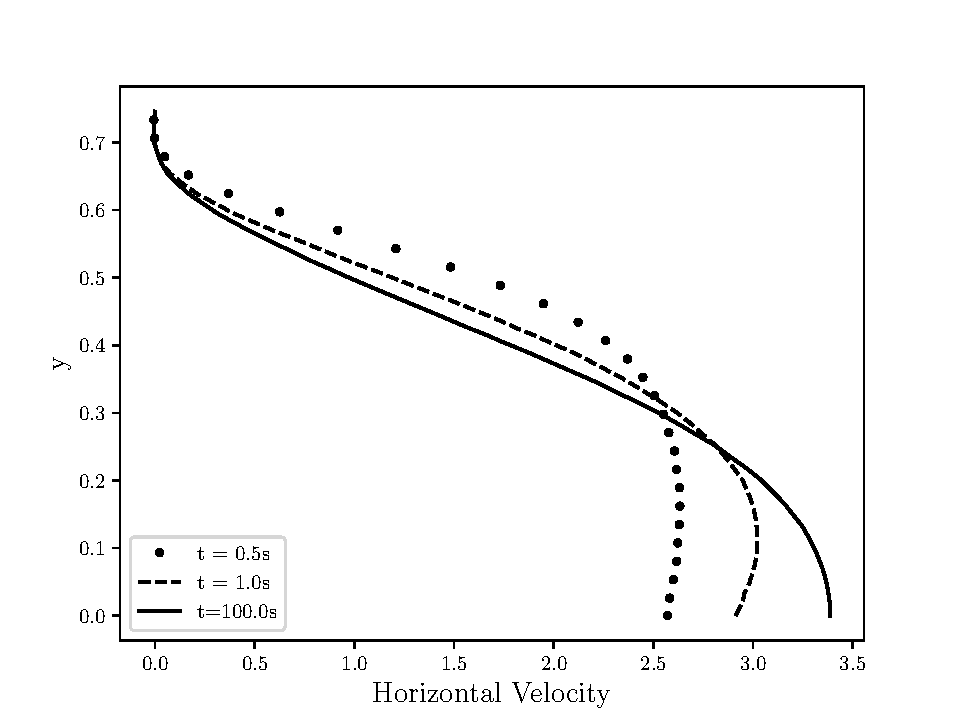
\includegraphics[scale=1]{./02_chaps/cap_solution/figure/vel_RealStrut_evol.pdf}\\
     \caption{Evolução no tempo do perfil da velocidade para o Canal Real com Stent Farmacológico.}
     \label{velocity evolution real stent}
\end{figure}

\newpage
A \ref{velocity field real stent} apresenta a evolução no tempo e no espaço
do campo de velocidade para a metade do domínio, pois os resultados são simétricos
na direção $y$. O campo de velocidade é representado com os valores adimensionais
onde a cor vermelha se refere ao valor $u=2.65$ e a cor azul $u=0$.
 
\vspace{2cm}
\begin{figure}[H]
     \begin{minipage}{.50\linewidth}
      \centering
      
\includegraphics[scale=0.12]{./02_chaps/cap_solution/figure/vel_RealStrut200.png}\\
      t = 0.1
     \end{minipage}%
     \begin{minipage}{.50\linewidth}
      \centering
      
\includegraphics[scale=0.12]{./02_chaps/cap_solution/figure/vel_RealStrut1000.png}\\
      t = 0.5
     \end{minipage}
     \begin{minipage}{.50\linewidth}
     \medskip
      \centering
      
\includegraphics[scale=0.12]{./02_chaps/cap_solution/figure/vel_RealStrut2000.png}\\
      t = 1.0
     \end{minipage}%
     \begin{minipage}{.50\linewidth}
     \medskip
      \centering
      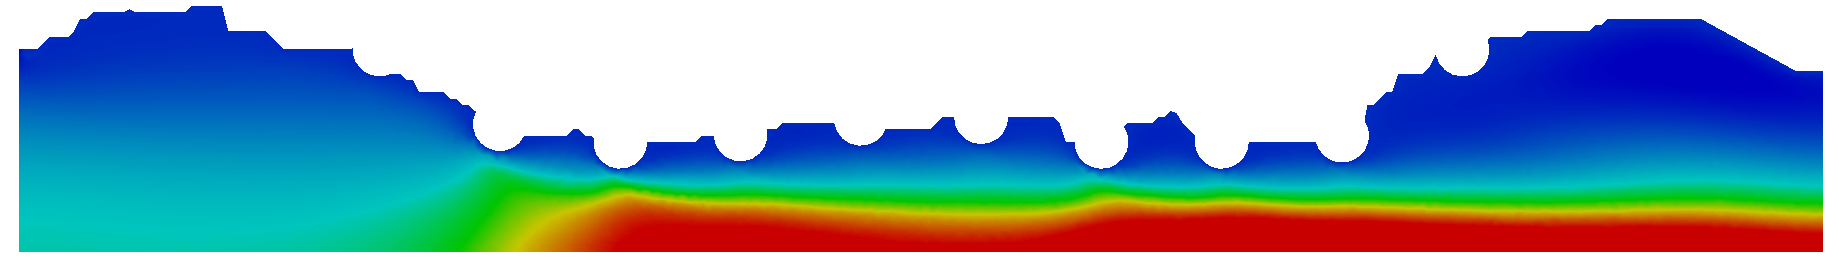
\includegraphics[scale=0.12]{./02_chaps/cap_solution/figure/vel_RealStrut6000.png}\\
      t = 3.0
     \end{minipage}
     \begin{minipage}{.50\linewidth}
      \centering
      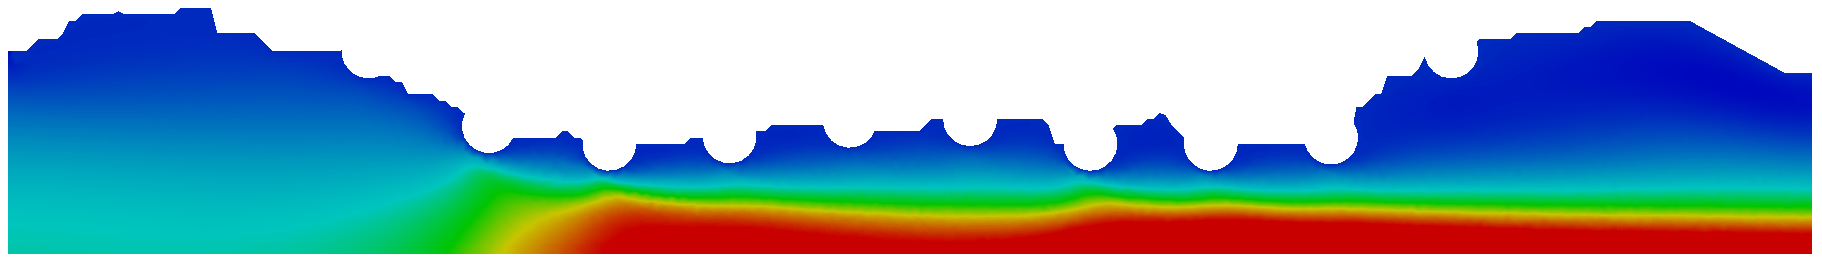
\includegraphics[scale=0.12]{./02_chaps/cap_solution/figure/vel_RealStrut8000.png}\\
      t = 4.0
     \end{minipage}%
     \begin{minipage}{.50\linewidth}
      \centering
      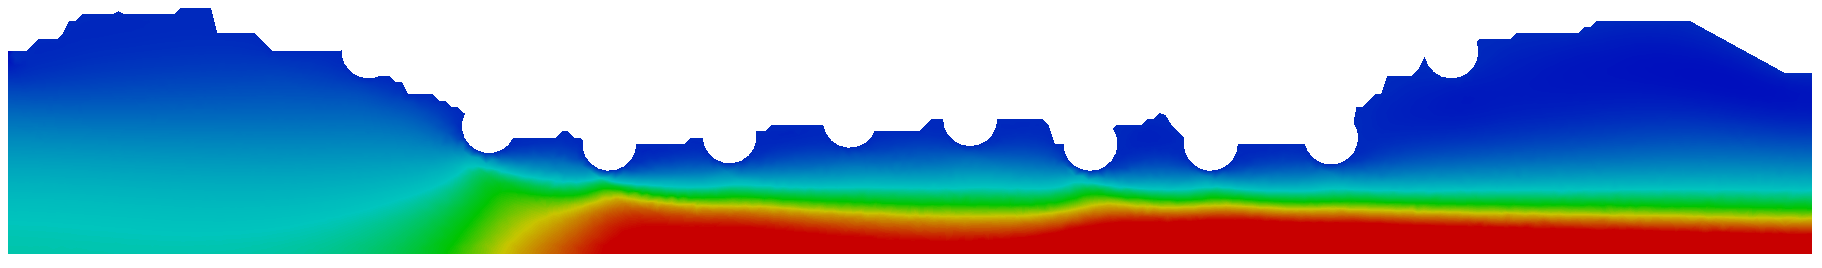
\includegraphics[scale=0.12]{./02_chaps/cap_solution/figure/vel_RealStrut10000.png}\\
      t = 5.0
     \end{minipage}
     \begin{minipage}{.50\linewidth}
     \medskip
      \centering
      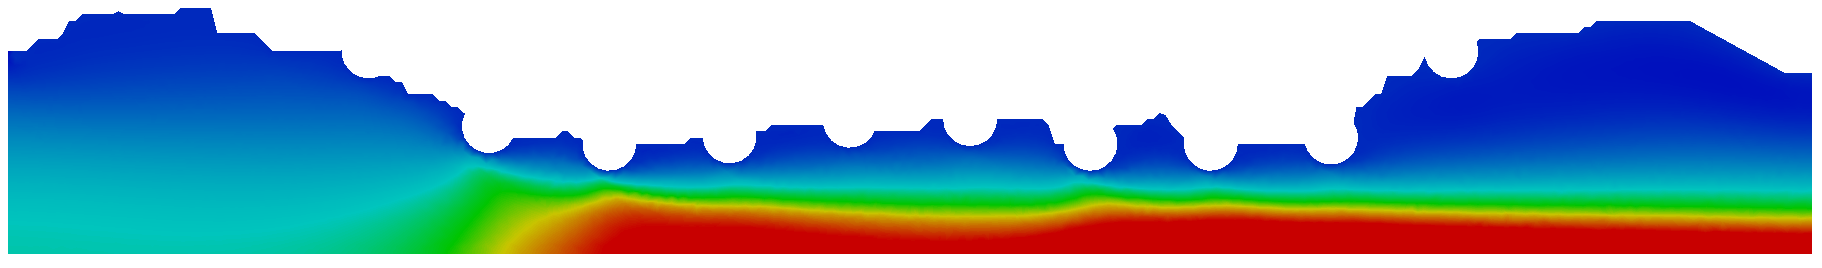
\includegraphics[scale=0.12]{./02_chaps/cap_solution/figure/vel_RealStrut14000.png}\\
      t = 7.0
     \end{minipage}%
     \begin{minipage}{.50\linewidth}
     \medskip
      \centering
      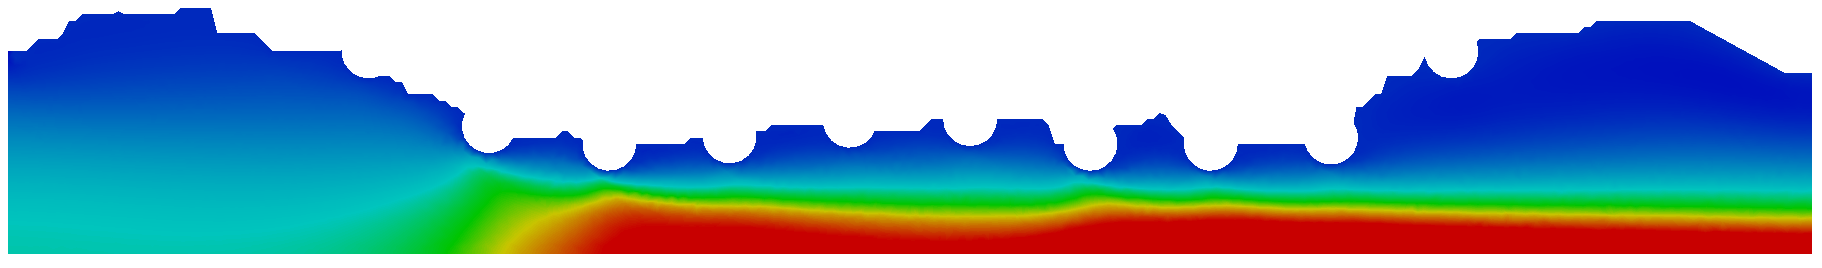
\includegraphics[scale=0.12]{./02_chaps/cap_solution/figure/vel_RealStrut20000.png}\\
      t = 10.0
     \end{minipage}
     \medskip
     \caption{Evolução no tempo e no espaço do campo de velocidade para o Canal Real com Stent Farmacológico.}
     \label{velocity field real stent}
\end{figure}

\vspace{1cm}
A \ref{conc field real stent sc 1} e a \ref{conc field real stent sc 10} 
apresentam a evolução no tempo e no espaço
do campo de concentração para a metade do domínio devido a simetria para diversos números de \textit{Schmidt}
tais como: $1$ e $10$, respectivamente. É possível observar a influência
do aumento do número de \textit{Schmidt} na difusão do fármaco.
A concentração é representada com os valores adimensionais
onde a cor vermelha representa $100$\% e a cor azul representa $0$\% 
da concentração que é difundida na corrente sanguínea. 


\begin{figure}[H]
     \begin{minipage}{.50\linewidth}
      \centering
      
\includegraphics[scale=0.12]{./02_chaps/cap_solution/figure/conc1_RealStrut200.png}\\
      t = 0.1
     \end{minipage}%
     \begin{minipage}{.50\linewidth}
      \centering
      
\includegraphics[scale=0.12]{./02_chaps/cap_solution/figure/conc1_RealStrut1000.png}\\
      t = 0.5
     \end{minipage}
     \begin{minipage}{.50\linewidth}
     \medskip
      \centering
      
\includegraphics[scale=0.12]{./02_chaps/cap_solution/figure/conc1_RealStrut2000.png}\\
      t = 1.0
     \end{minipage}%
     \begin{minipage}{.50\linewidth}
     \medskip
      \centering
      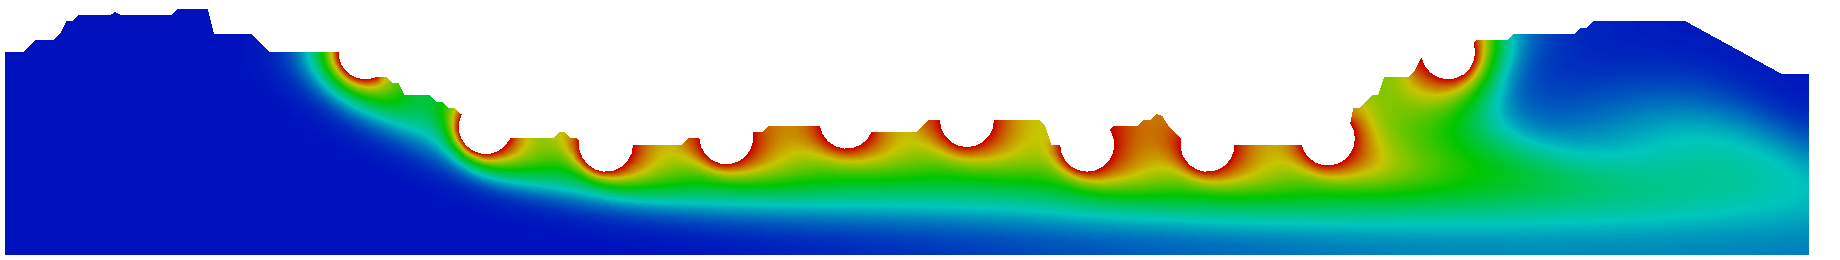
\includegraphics[scale=0.12]{./02_chaps/cap_solution/figure/conc1_RealStrut6000.png}\\
      t = 3.0
     \end{minipage}
     \begin{minipage}{.50\linewidth}
      \centering
      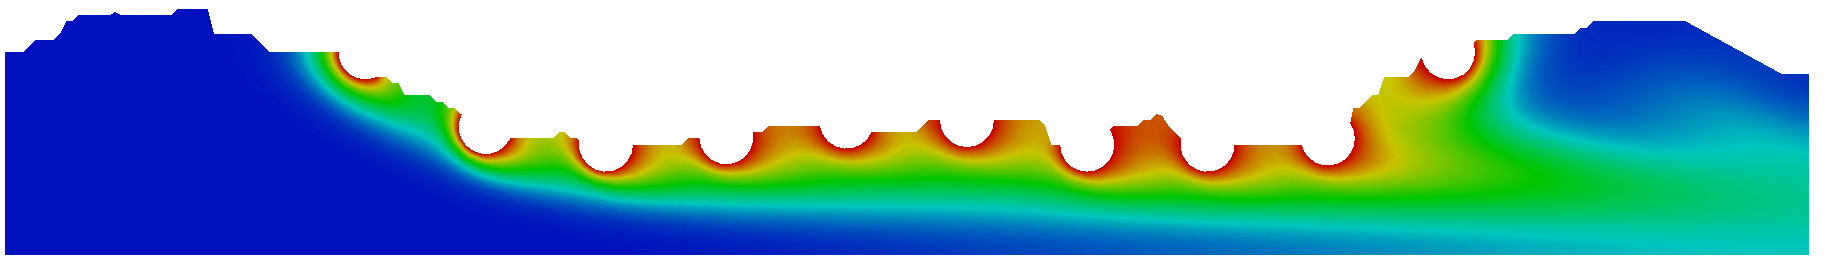
\includegraphics[scale=0.12]{./02_chaps/cap_solution/figure/conc1_RealStrut8000.png}\\
      t = 4.0
     \end{minipage}%
     \begin{minipage}{.50\linewidth}
      \centering
      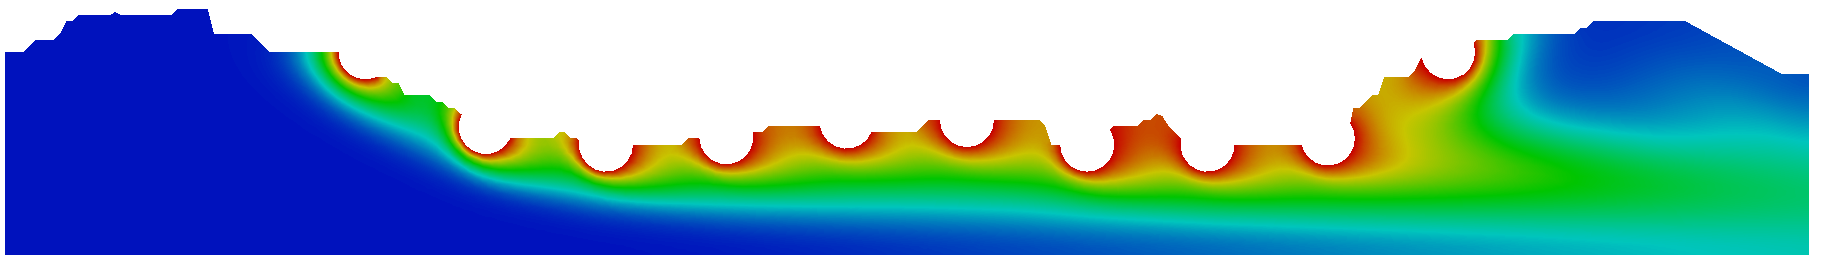
\includegraphics[scale=0.12]{./02_chaps/cap_solution/figure/conc1_RealStrut10000.png}\\
      t = 5.0
     \end{minipage}
     \begin{minipage}{.50\linewidth}
     \medskip
      \centering
      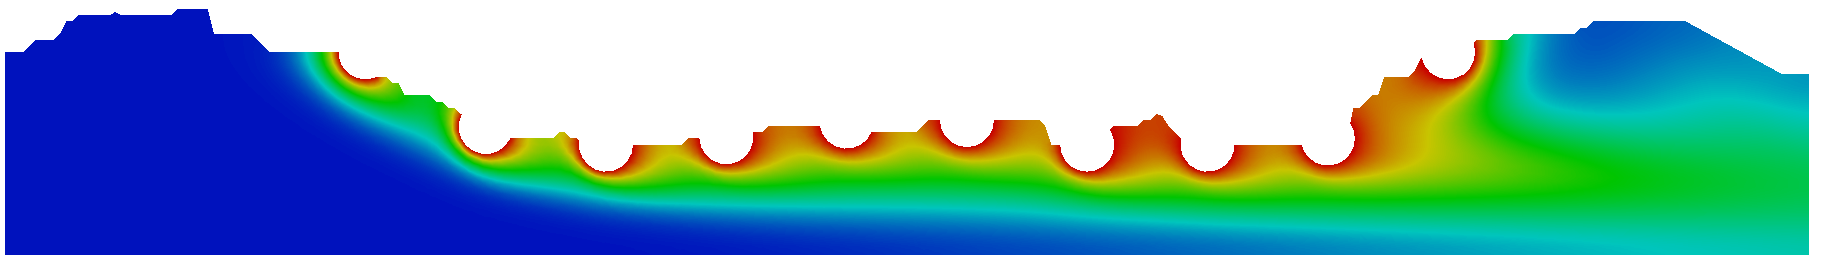
\includegraphics[scale=0.12]{./02_chaps/cap_solution/figure/conc1_RealStrut14000.png}\\
      t = 7.0
     \end{minipage}%
     \begin{minipage}{.50\linewidth}
     \medskip
      \centering
      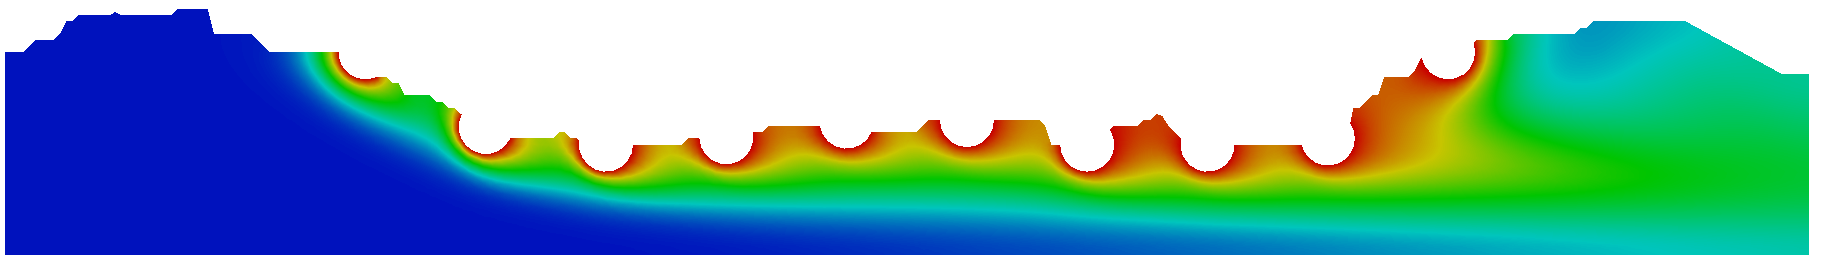
\includegraphics[scale=0.12]{./02_chaps/cap_solution/figure/conc1_RealStrut20000.png}\\
      t = 10.0
     \end{minipage}
     \medskip
     \caption{Evolução no tempo e no espaço do campo de espécie química para o Canal Real com Stent Farmacológico com $Sc=1$.}
     \label{conc field real stent sc 1}
\end{figure}

\bigskip
\begin{figure}[H]
     \begin{minipage}{.50\linewidth}
      \centering
      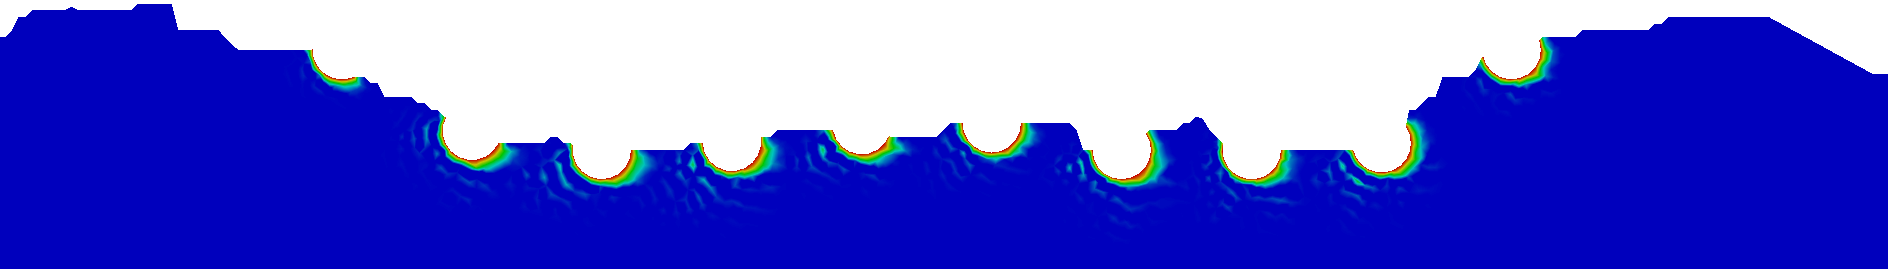
\includegraphics[scale=0.115]{./02_chaps/cap_solution/figure/conc10_RealStrut500.png}\\
      t = 0.1
     \end{minipage}%
     \begin{minipage}{.50\linewidth}
      \centering
      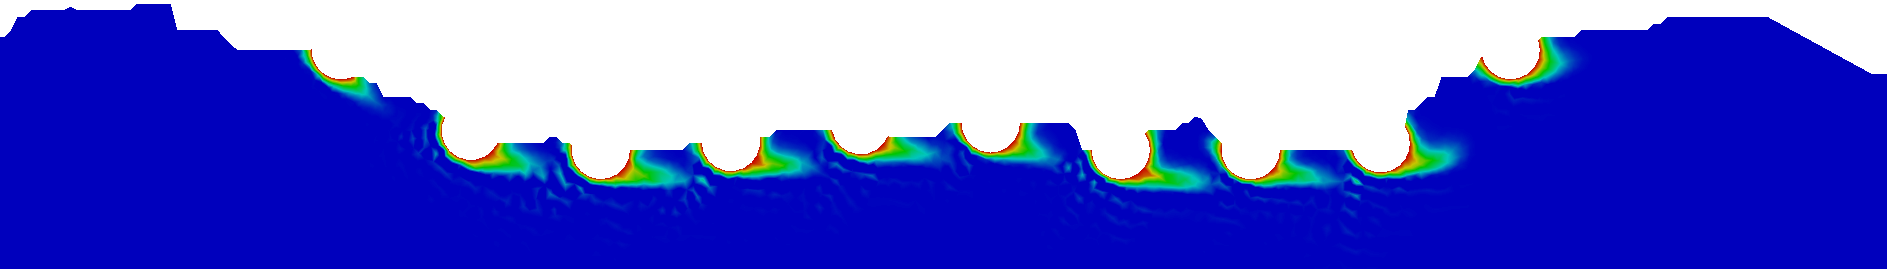
\includegraphics[scale=0.115]{./02_chaps/cap_solution/figure/conc10_RealStrut2500.png}\\
      t = 0.5
     \end{minipage}
     \begin{minipage}{.50\linewidth}
     \medskip
      \centering
      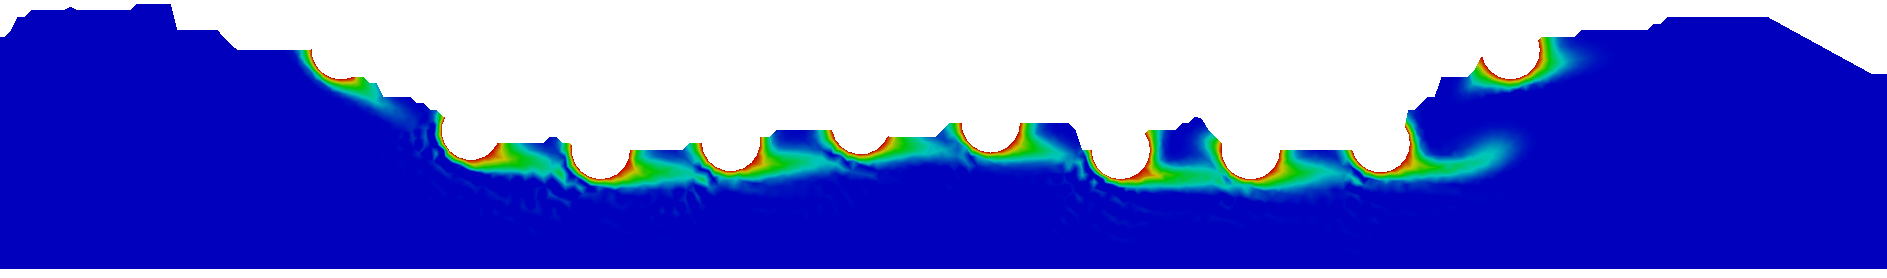
\includegraphics[scale=0.115]{./02_chaps/cap_solution/figure/conc10_RealStrut5000.png}\\
      t = 1.0
     \end{minipage}%
     \begin{minipage}{.50\linewidth}
     \medskip
      \centering
      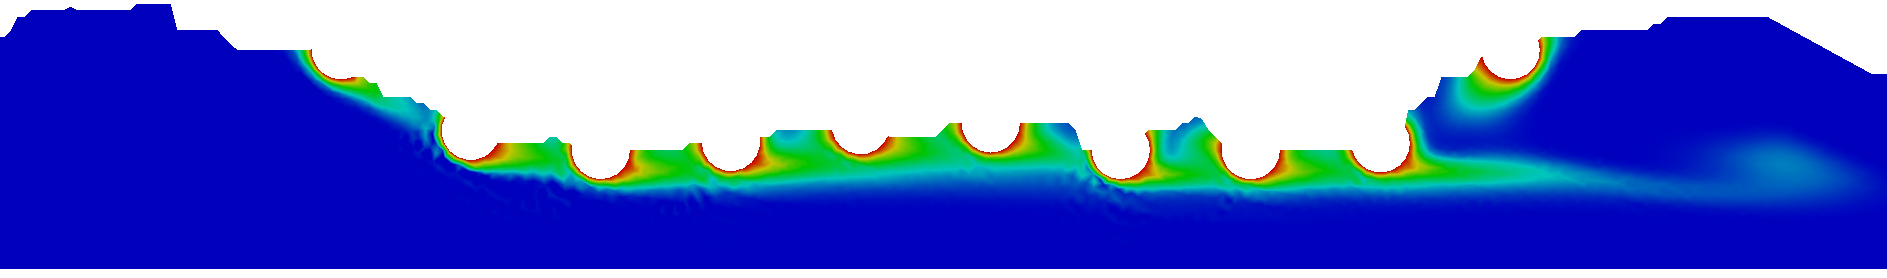
\includegraphics[scale=0.115]{./02_chaps/cap_solution/figure/conc10_RealStrut15000.png}\\
      t = 3.0
     \end{minipage}
     \begin{minipage}{.50\linewidth}
      \centering
      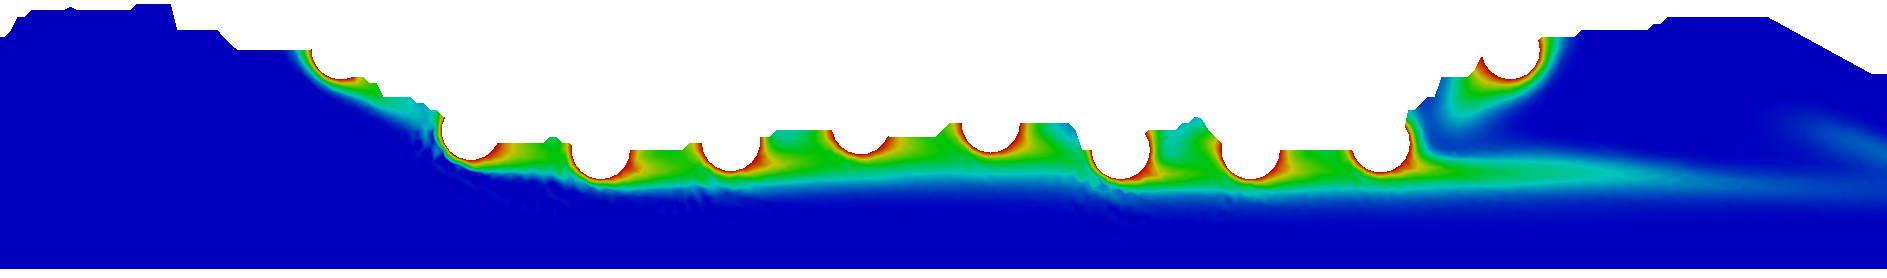
\includegraphics[scale=0.115]{./02_chaps/cap_solution/figure/conc10_RealStrut20000.png}\\
      t = 4.0
     \end{minipage}%
     \begin{minipage}{.50\linewidth}
      \centering
      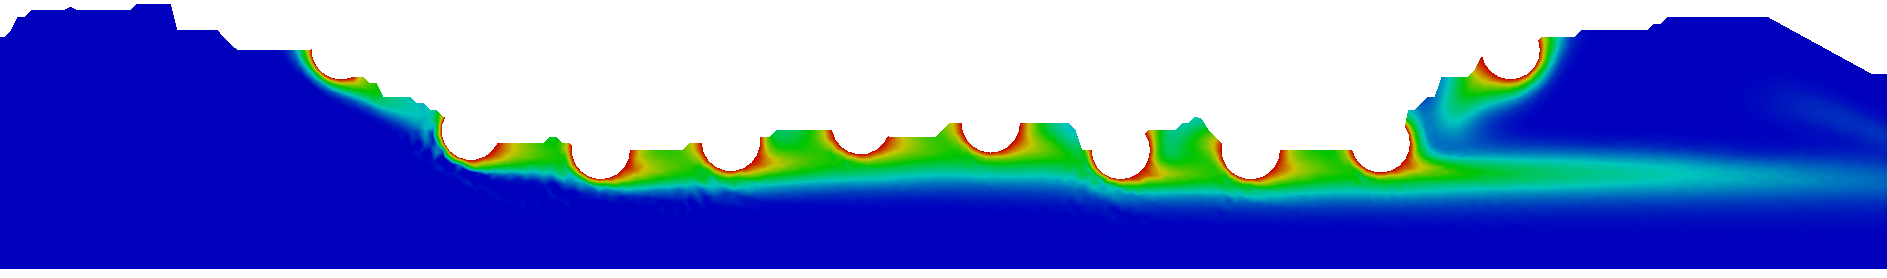
\includegraphics[scale=0.115]{./02_chaps/cap_solution/figure/conc10_RealStrut25000.png}\\
      t = 5.0
     \end{minipage}
     \begin{minipage}{.50\linewidth}
     \medskip
      \centering
      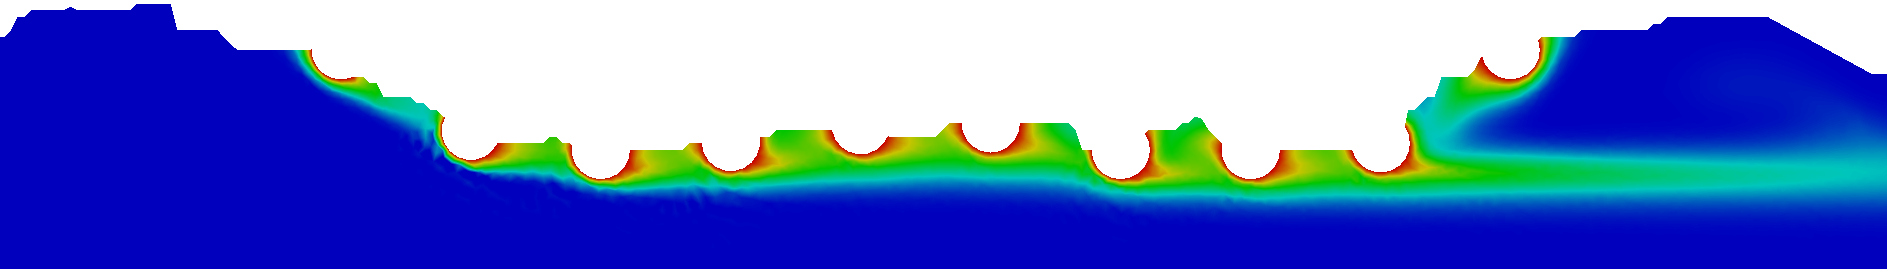
\includegraphics[scale=0.115]{./02_chaps/cap_solution/figure/conc10_RealStrut35000.png}\\
      t = 7.0
     \end{minipage}%
     \begin{minipage}{.50\linewidth}
     \medskip
      \centering
      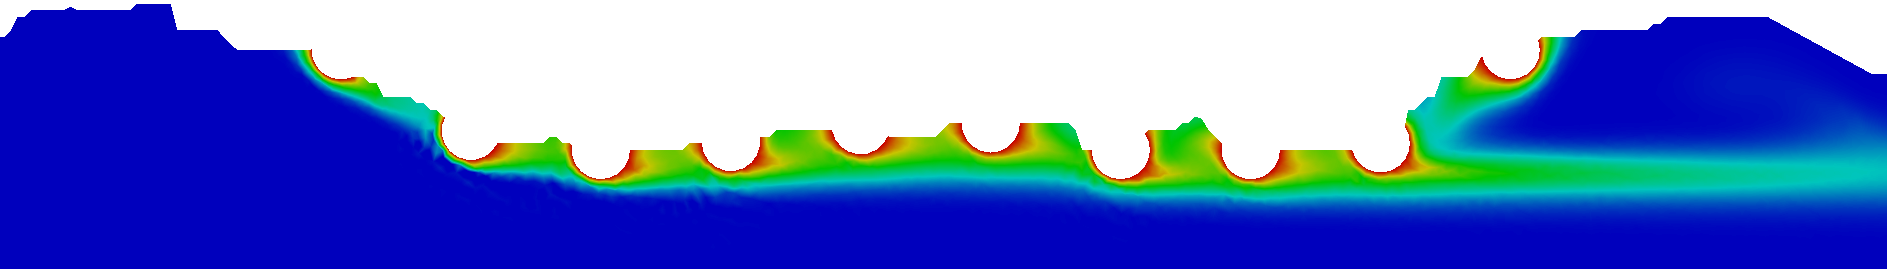
\includegraphics[scale=0.115]{./02_chaps/cap_solution/figure/conc10_RealStrut50000.png}\\
      t = 10.0
     \end{minipage}
     \medskip
     \caption{Evolução no tempo e no espaço do campo de espécie química para o Canal Real com Stent Farmacológico com $Sc=10$.}
     \label{conc field real stent sc 10}
\end{figure}


\newpage


